\documentclass[11pt,letterpaper]{article}

% ---------- Page geometry ----------
\usepackage[margin=1in]{geometry}

% ---------- Encoding and fonts ----------
\usepackage[T1]{fontenc}
\usepackage[utf8]{inputenc}
\usepackage{lmodern}
\usepackage{microtype}

% ---------- Math ----------
\usepackage{amsmath, amssymb, amsthm, mathtools}

% ---------- Graphics, color, tables ----------
\usepackage{graphicx}
\usepackage{xcolor}
% Required by the figures in figures/ (architecture, training-ladder,
% episode-timeline); uncomment together with their \input lines in
% sections/method.tex and sections/training.tex.
\usepackage{tikz}
\usetikzlibrary{arrows.meta,positioning,fit,backgrounds,shapes.misc}
\usepackage{booktabs}
\usepackage{array}
\usepackage{enumitem}

% ---------- Algorithms ----------
\usepackage{algorithm}
\usepackage{algpseudocode}

% ---------- Links and citations ----------
\usepackage[colorlinks=true, allcolors=blue]{hyperref}
\usepackage[numbers, sort&compress]{natbib}
\usepackage[capitalize]{cleveref}

% ---------- Draft status marker ----------
% Scaffold discipline: sections marked [STUB] await the LLMContextMDP
% integration (method mechanics) or experimental runs (results). Do not
% present stubbed content as complete. Source of truth for the method is
% design.md at the repository root.
\newcommand{\stub}[1]{\textcolor{red!70!black}{[STUB: #1]}}

\title{Verifier-Anchored Reinforcement Learning:\\
A Tiny Learned Controller Orchestrating a Frozen Language Model\\
over a Structured Reasoning State}

\author{
  Alexander Towell\\
  Southern Illinois University Edwardsville\\
  \texttt{atowell@siue.edu}
}

\date{Draft scaffold, \today. Results pending.}

\begin{document}

\maketitle

\begin{abstract}
We present a reinforcement-learning framework for training small language
models to reason on verifiable problems. The agent performs approximate
$Q$-learning over an LLM-induced context Markov decision process: states are
structured contexts, actions are a small set of coarse cognitive verbs the
model realizes as text, transitions are sampled from the model's responses,
and reward is anchored by a non-LLM verifier (a symbolic solver, unit-test
harness, or proof checker) rather than a learned critic. The action-value
function $\Qpsi(s, a)$ is a multi-head $Q$-network over the hidden state of a
frozen base model. Monte Carlo Tree Search enters not as the core learning
algorithm but as a policy-improvement operator: it produces locally improved
estimates $\Qmcts(s, a)$ and visit-count policies $\pimcts$ that serve as
stronger training targets for expert iteration, and it doubles as a
test-time-compute knob at inference. Keeping reward verifier-anchored rather
than learned reduces the Goodhart attack surface. We give the framework, the
architecture, and a pre-registered experimental plan with falsifiable
hypotheses (a fixed baseline grid, a FLOP-accounted compute axis, and a
Holm-Bonferroni-corrected criterion committed before training), plus a
toy-problem pilot. One round of expert iteration raises zero-shot held-out
argmax agreement by $15$ percentage points ($57\% \to 72\%$, single training
seed); a second round on naively-expanded data yields a structurally
informative regression that a controlled rebalancing test traces to
distillation-target instability rather than class dilution. We then run the
full online loop on an in-process $1.5$B substrate: a first closed-loop run
establishes the honest per-decision compute accounting, and a fully
instrumented run capturing the $Q$-loss trend and prior-sharpening signal
across iterations is currently executing, with those results pending. The
pilot is feasibility evidence; the large-scale benchmark claim is deferred to
a follow-up study.
\end{abstract}


\section{Introduction}
\label{sec:introduction}

\paragraph{Motivation.}
A central trend in large language model deployment is the explicit allocation
of test-time compute to deliberation. Modern reasoning systems such as
OpenAI's o1 line \citep{openai2024o1} and the public scaling analyses of
\citet{snell2024scaling} demonstrate that, for verifiable problems,
additional inference-time computation can yield accuracy gains comparable to
those produced by orders-of-magnitude increases in pretraining scale. At the
same time, small open-weight models, on the order of one to seven billion
parameters, lag far behind frontier reasoning models on mathematical and
programmatic benchmarks such as GSM8K \citep{cobbe2021gsm8k} and MATH
\citep{hendrycks2021math}, even when given generous decoding budgets. The
gap is widest precisely where it should be most closable: on problems whose
solutions can be checked by a non-LLM verifier such as a symbolic algebra
system, a unit-test harness, or a proof assistant. Whenever a cheap and
trustworthy verifier exists, the loop from candidate solution to scalar reward
is short, dense, and not subject to reward hacking by a learned critic
\citep{lightman2024verify}. This is the classical setting in which
reinforcement learning excels.

We therefore frame the problem squarely as reinforcement learning. The agent
interacts with an environment whose dynamics are induced by a base language
model and whose terminal reward is supplied by an external verifier. Learning
proceeds by approximate $Q$-learning over sampled transitions, in the
direct lineage of \citet{sutton2018reinforcement} and the deep $Q$-learning
techniques of \citet{mnih2015human}. The natural question is then whether a
small base model, paired with a learned action-value function trained against
verifier-anchored Bellman targets, can close a meaningful fraction of the gap
to much larger reasoning models on a fixed compute axis. This paper is the
methodological prerequisite to answering that question.

\paragraph{Position.}
This is a methodology paper with a toy-problem pilot. We make the framework
precise enough to be evaluated as a contribution in its own right, we
pre-register the experimental design so that the eventual benchmark study
will not be confused with post-hoc rationalization, and we report a
small-scale pilot that exercises the full pipeline end-to-end and demonstrates
that the expert-iteration loop closes under the framework's implementation.
The pilot is not a benchmark study: it tests feasibility on four toy problems
under a single base model and a small MCTS budget, with the goal of falsifying
the framework's basic mechanics before the large benchmark study begins.
Concretely, we present a reinforcement-learning framework specialized for
verifiable LLM-induced context Markov decision processes, an architecture
that uses a shared frozen language model as both encoder and stochastic
transition model, a reward structure that quarantines learned aesthetic
signals away from the Bellman target, an explicit role for tree search as a
policy improvement operator rather than as the central learning algorithm,
a pre-registered evaluation plan with falsifiable hypotheses against
standardized benchmarks, and a toy-problem pilot whose positive and
informatively-negative findings are reported alongside the framework.

The reframing relative to prior MCTS-centric work is deliberate. In the
AlphaZero tradition \citep{silver2017alphagozero, silver2018alphazero} and its
expert-iteration ancestor \citep{anthony2017thinking}, tree search is the
narrative center and the learned policy is its student. In our setting the
center is the agent and its action-value function $\Qpsi(s, a)$. Tree search
is one of several mechanisms for producing better samples and stronger
training targets. This shift in emphasis has practical consequences: it makes
non-search baselines such as $\epsilon$-greedy and softmax exploration first-class
citizens, it clarifies what the verifier is for, and it makes the test-time
search knob optional rather than load-bearing.

\paragraph{Contributions.}
We make six contributions:
\begin{enumerate}[leftmargin=*]
  \item A reinforcement-learning framework that casts LLM deliberation on
        verifiable tasks as an approximate $Q$-learning problem over an
        induced context MDP, with a structured state schema
        (Section~\ref{sec:method-state}) that makes the Markov bet explicit
        and a canonical \textsc{InvokeVerifier} action that is part of
        the agent's action space rather than a post-hoc parser pass.
  \item An architecture that uses a single frozen base language model as both
        encoder and stochastic transition model, with a small adapter and a
        multi-head parametric action-value network $\Qpsi(s, a)$ over a fixed
        verb set (Section~\ref{sec:method-architecture}). The choice of a
        multi-head $Q$ over a fixed action set, rather than a scoring head over
        $(s, a)$ embeddings, is justified by the available action cardinality
        and by the gradient-routing properties of the architecture.
  \item A reward-design principle that separates verifier-anchored Bellman
        targets from learned-aesthetic signals
        (Section~\ref{sec:method-reward}). Verifier outcomes form the external
        reward and the Bellman backup; learned signals such as
        reasoning-quality classifiers or deception detectors may enter only as
        search priors, never as reward, reducing the Goodhart attack surface.
  \item Monte Carlo Tree Search as a sample-efficient policy improvement
        operator (Section~\ref{sec:method-mcts}), producing stronger training
        targets $\Qmcts(s, a)$ and a visit-count policy $\pimcts$ that are
        distilled into the parametric $Q$ and policy heads. The same operator
        serves as a test-time-compute knob at inference: a fast greedy mode
        evaluates $\Qpsi$ once per state, while a search mode invokes MCTS
        when latency permits. Search is therefore an optional accelerator,
        not the central learning algorithm.
  \item A pre-registered evaluation plan
        (Section~\ref{sec:experimental-plan}) that defines the baseline grid,
        the compute axis, and the headline compute-versus-accuracy frontier
        figure before any training begins, with falsifiable hypotheses and an
        explicit threat model for compute leaks in test-time-compute claims.
  \item A toy-problem pilot (Section~\ref{sec:pilot}) that exercises every
        component of the framework end-to-end across two rounds of expert
        iteration plus a controlled rebalancing test, demonstrates that a
        single round improves zero-shot held-out argmax agreement by $15$
        percentage points ($57\% \to 72\%$) and reduces mean $L_1$ to MCTS
        targets by $42\%$, and dissects a second-round regression: the
        rebalancing test rules out class dilution as the dominant
        mechanism, surfacing target-stability and shortcut-dependence
        constraints that the pre-registered benchmark study inherits as
        monitoring requirements.
\end{enumerate}

\paragraph{Paper structure.}
Section~\ref{sec:background} develops the reinforcement-learning background:
Markov decision processes, the Bellman optimality equation, tabular and
approximate $Q$-learning with target networks, exploration policies, and MCTS
as a policy improvement operator in the AlphaZero tradition, ending with the
LLM-induced context MDP framing. Section~\ref{sec:method} presents the
framework in detail: the state schema, the action space including the verifier
action, the shared-encoder architecture, the role of MCTS in producing
training targets and at inference, the reward structure, the training loop
combining replay-based approximate $Q$-learning with expert-iteration
distillation, and the two inference modes.
Section~\ref{sec:experimental-plan} specifies the experimental design and the
hypotheses to be tested. Section~\ref{sec:pilot} reports the toy-problem
pilot: setup, the improvement from the first round of expert iteration, the
informatively-negative regression of the second round, a controlled
rebalancing test that isolates the regression's mechanism, and the design
implications carried forward into the pre-registered study.
Section~\ref{sec:related-work} positions the contribution against prior work
in classical RL, verifier-supervised reasoning, test-time-compute scaling,
MCTS-augmented language models, and small-model self-improvement.
Section~\ref{sec:discussion} discusses limitations, extensions, and threats
to validity. Section~\ref{sec:conclusion} concludes.

\section{Related Work}
\label{sec:related-work}

% =========================================================================
% Five subsections, each one to two paragraphs of drafted prose.
% Framework is positioned as approximate Q-learning over a verifier-
% anchored context MDP, with MCTS as a policy improvement operator and
% a test-time-compute knob, not as MCTS-first.
% =========================================================================

\subsection{Search and Learning in Games}
\label{sec:rw-games}

The conceptual ancestor of the present framework is the joint use of tree
search and learned function approximation in self-play games. UCT
\citep{kocsis2006bandit} and the original Monte Carlo tree search of
\citet{coulom2006efficient} supplied the algorithmic backbone; the broader
landscape of variants and applications is surveyed by
\citet{browne2012survey}. The AlphaGo family
\citep{silver2016alphago, silver2017alphagozero, silver2018alphazero}
combined deep neural priors and value estimates with PUCT-guided search,
distilling the search policy back into the priors in a closed loop. MuZero
\citep{schrittwieser2020muzero} extended the same recipe to settings whose
dynamics must be learned. The expert-iteration formulation of
\citet{anthony2017thinking} states the underlying pattern abstractly: a
fast \textit{apprentice} policy is improved by an expensive \textit{expert}
operator (search), and the apprentice is then trained to imitate the
expert's behavior.

We inherit this joint search-and-learning structure but invert the
narrative emphasis. In the AlphaZero tradition, tree search is the central
object and the learned heads are its scaffolding; in our setting the
central object is an agent and its approximate action-value function
$\Qpsi(s, a)$, trained against verifier-anchored Bellman targets, and
search enters as one of several mechanisms that supply stronger training
targets and an optional test-time-compute knob
(Sections~\ref{sec:method-training} and~\ref{sec:method-inference}). The
shift is what is appropriate when (a) the environment is stochastic and
LLM-induced rather than a deterministic two-player game, so a chance-node
estimator becomes essential and a collapsed single-node tree becomes
biased (Section~\ref{sec:method-mcts}); and (b) the value channel is
anchored by a non-LLM verifier rather than by game outcomes alone, which
makes a wider set of non-search exploration policies viable as baselines
and makes the choice between $\epsilon$-greedy, softmax, and search-driven
data collection an empirical rather than an architectural question.

\subsection{Verifier-Anchored LLM Reasoning}
\label{sec:rw-verifiers}

Several recent systems share the principle that learning signal for
reasoning models should come from non-LLM verifiers rather than from
human-rated aesthetic critics. \citet{lightman2024verify} demonstrated
that process reward models trained on per-step labels for MATH solutions
outperform outcome-only supervision on the same benchmark, and
\citet{cobbe2021gsm8k} introduced GSM8K together with the original
verifier-style training pipeline for grade-school arithmetic. AlphaCode
\citep{li2022alphacode} used unit-test execution as the verifier for
competitive programming, and AlphaProof \citep{deepmind2024alphaproof}
extended the same architectural pattern to formal mathematics with Lean
as the verifier. \citet{guo2025deepseekr1} report large-scale
reinforcement learning against rule-based verifiers for math and code
without a learned reward model, deliberately avoiding the Goodhart
attack surface that attends preference-trained critics.

Our work shares the verifier-anchored reward principle but contributes
along two axes. The first is framework-level: Section~\ref{sec:method-reward}
makes the verifier-versus-aesthetic asymmetry a load-bearing design
commitment rather than an implementation detail. Verifier outcomes are the
only signals allowed to enter the Bellman target; learned aesthetic
signals such as reasoning-quality classifiers or deception detectors may
enter only as MCTS priors, where they bias exploration but cannot rewrite
the value function. The second is architecture-level:
$\textsc{InvokeVerifier}$ is a callable verb in the agent's action space
(Section~\ref{sec:method-actions}) rather than a post-hoc parser pass
applied only at the terminal answer. The agent decides when to spend a
verifier call, intermediate verifier outputs land in the structured state
and become available to the heads, and a hypothesis can be promoted to a
verified fact mid-trajectory. The choice converts verifier interaction
from a wrapper around the model into a first-class part of the
deliberation, which is what makes verifier-anchored intermediate rewards
(Equation~\ref{eq:rewardterminal} and the fallback discussion that
follows it) consistent with the no-Goodhart principle.

\subsection{Test-Time Compute Scaling}
\label{sec:rw-ttcs}

\citet{snell2024scaling} established empirical scaling laws relating
test-time compute to accuracy on verifiable benchmarks, showing that
optimal inference-time allocation can match or exceed the returns of
proportional pretraining-scale increases. OpenAI's o1 line
\citep{openai2024o1} is the public anchor for test-time-compute-as-product
in deployed reasoning systems. A common pattern in this literature is the
inference-time technique (chain-of-thought \citep{wei2022cot},
self-consistency, best-of-$N$, beam search over rationales) studied as a
post-hoc augmentation of an already-trained generator.

Our contribution is methodological rather than algorithmic in this
register. Section~\ref{sec:exp-baselines} pre-registers a baseline grid
that separates fast-mode policy improvement ($B = 0$, where the trained
$Q$-head is acted on greedily) from search-mode improvement ($B > 0$,
where MCTS refines the head estimate at the query), with matched
inference compute across all conditions. The separation matters because
the literature has often conflated two distinct claims: ``the model is
better at compute $X$'' (which can be true purely because the trained
heads are stronger) and ``the model uses additional compute $X$
usefully'' (which is the genuine test-time-compute question). By writing
the compute axis, the baseline grid, and the headline frontier figure
before any training begins, we make the conflation difficult to commit
in either direction. The same evaluation protocol turns the search budget
$B$ from a tuned hyperparameter into a continuous dial the user
controls at inference, which is the practically relevant form of a
test-time-compute knob.

\subsection{MCTS for Language Model Reasoning}
\label{sec:rw-mcts-llm}

A growing body of recent work applies tree search to language model
reasoning. \citet{feng2023alphazerollm} adapt the AlphaZero recipe
directly, using a learned value model and PUCT to guide token-level or
step-level decoding. \citet{xie2024monte} use MCTS to generate preference
data for iterative DPO-style training, treating search as a trajectory
generator whose output is consumed downstream. The closest prior
published system to our framework is rStar-Math
\citep{guan2025rstarmath}, which combines small base language models
with MCTS-based self-training and a process reward model trained from
MCTS rollouts; the broad approach (small LMs, search-guided rollouts,
distillation from search statistics) is the same family our framework
inhabits, and rStar-Math's empirical results establish that the family
works on competition-grade math. The general shape of these systems is
recognizable from the AlphaZero ancestor: tree search produces better
trajectories than the base policy, and the base policy is updated toward
what search would have done.

Our work differs along four structural axes that together distinguish a
framework paper from a fitted system. First, the search tree explicitly
bifurcates decision and chance nodes (Section~\ref{sec:method-mcts}); this
is what makes the chance-node mean $W(s, a) / N(s, a)$ a legitimate
estimator of the inner Bellman expectation when the environment is
stochastic, as it is whenever the transition is induced by LLM sampling
rather than by deterministic game rules. Collapsing the two node types,
the pattern most often seen in deterministic-game tutorials, biases every
ancestor's $Q$-estimate. Second, the agent acts over a small fixed set of
coarse verbs $\Aset$ (Section~\ref{sec:method-actions}) and the
$Q$-function is a multi-head categorical output rather than a scorer over
$(s, a)$ embeddings of free-form text. This trades expressivity for a
stable categorical distribution that PUCT can branch on and that the
policy head can match by cross-entropy. Third, $\textsc{InvokeVerifier}$
is one of the verbs the agent may take rather than a step performed only
on the committed answer (Section~\ref{sec:method-actions}); the verifier
is a learnable resource the policy budgets. Fourth, the architecture,
action space, evaluation protocol, and falsifiable hypotheses are
pre-registered (Section~\ref{sec:experimental-plan}) before any training
begins, which is what we take to distinguish a methodology paper from a
post-hoc justification of an empirically tuned system.

Two of these axes deserve specific contrast with
\citet{guan2025rstarmath}. On the state and action axis, rStar-Math
operates over token-level or step-level decoding, with search nodes
keyed to partial generations of natural-language reasoning; our context
MDP is a structured-state object with a fixed seven-verb action space
and id-based targeting (Sections~\ref{sec:method-state}
and~\ref{sec:method-actions}), so the categorical action set is small
and stable across problems and chance nodes can be addressed by
identifier rather than by string match. On the methodology axis,
rStar-Math is a fitted system whose architectural choices, reward
shaping, and evaluation protocol are reported alongside its empirical
results; our framework pre-registers the baseline grid, statistical
analysis plan, and falsifiable hypotheses (Section~\ref{sec:experimental-plan})
before training begins. The two efforts are complementary: rStar-Math
demonstrates empirically that small base LMs with MCTS-driven
self-training reach competitive math accuracy, and our framework aims
to make the design space and the falsification criteria of that broad
approach explicit.

\subsection{Self-Improvement and Synthetic Trajectory Generation}
\label{sec:rw-selfimprove}

A complementary line of work asks whether a language model can improve
itself by generating its own training data. STaR \citep{zelikman2022star}
samples rationales from the base model, retains those whose final answer
matches a known label, and fine-tunes on the retained set; the procedure
is iterated. V-STaR \citep{hosseini2024vstar} trains a verifier on the
rationales STaR discards and uses it at inference to rerank candidates.
Both approaches operate at the granularity of complete trajectories: the
unit of credit is the whole solution path, and the supervision signal is
whether the path's final answer is correct.

Our framework sits in the same family of search-then-distill systems but
distills at a finer granularity. MCTS produces locally improved
trajectories, and the heads are trained on per-step chance-node estimates
$\Qmcts(s, a)$ rather than only on terminal correctness
(Section~\ref{sec:method-training}). What makes per-step distillation
feasible is the structured intermediate state of
Section~\ref{sec:method-state}: a math state with explicit
\texttt{Fact}, \texttt{Subgoal}, \texttt{Hypothesis}, and verifier-call
records is a Markov state with a well-defined value, whereas a raw
token-prefix has neither. The per-step credit assignment is closer to
classical $Q$-learning than to trajectory-level rejection sampling: the
chance-node $Q$-estimate at $(s, a)$ averages over the discounted return
of every continuation that branches from that action, so a correct
intermediate hypothesis that leads to an incorrect final commit still
receives a positive partial-credit signal at the chance node where it was
introduced. The structural-state choice is therefore what allows the
search-then-distill pattern of STaR's lineage to be carried over into a
Bellman-style update rather than a trajectory-level supervised target.

\section{Method: A Lens-Structured Context MDP}
\label{sec:method}

We formulate deliberation as a finite-horizon discounted MDP
$(S, A, P, R, \gamma)$ induced by a frozen language model: $S$ the set of
reasoning-forest states, $A$ the typed actions of
\cref{sec:method-actions}, $P(s' \mid s, a)$ the transition probability
(sampled, never enumerated, because it integrates over the frozen model's
continuations), $R(s, a, s')$ the reward of \cref{sec:method-reward}, and
$\gamma \in (0, 1]$ the discount factor. Episodes run for at most
$T_{\max}$ turns (the depth limit). This section
specifies the state (\cref{sec:method-state}), the action space and lens
semantics (\cref{sec:method-actions}), the controller network
(\cref{sec:method-controller}), and the reward (\cref{sec:method-reward}).
Training is deferred to \cref{sec:training}.

\subsection{State: an immutable reasoning forest}
\label{sec:method-state}

The state is an immutable forest of typed nodes: \emph{goals} (the problem
is the root; subgoals are optional decompositions), \emph{hypotheses}
(tentative claims attached to a goal), \emph{facts} (claims with provenance
\texttt{given}, \texttt{derived}, or \texttt{verified}), and
\emph{verifier-call records} (the input, output, and success flag of each
call to the symbolic oracle, retained as part of the state). Every action
returns a new state; nodes carry stable integer identifiers so actions can
reference them.

Two properties are load-bearing. First, the distinction between
\emph{verified facts} and \emph{tentative hypotheses} is what gives
\textsc{Verify} its meaning: without it the controller cannot distinguish
``I proved this'' from ``I think this.'' Predicates such as
\textit{solved} and \textit{verified} are \emph{derived} from the
structure; they are information the policy may read, never a control-flow
constraint. Second, decomposition is \emph{optional scaffolding}: the policy
may split a goal, work on some children, ignore others, abandon a branch, or
commit the root directly from a single verified hypothesis. The only hard
gate in the system is the verifier-vouched witness check at commit time.
Connectives on decomposition edges (conjunctive versus exhaustive-case) are
recorded as non-gating metadata; whether checked aggregation helps is an
ablation, deferred with the move from answer verification to proof
verification.

A worked forest for $|x-3| + |x+2| = 7$ by case analysis, exercising every
node kind and both closure polarities, is:

{\small
\begin{verbatim}
GOAL solve |x-3| + |x+2| = 7          (root; connective: exhaustive_case)
+- GOAL case x < -2:   -(x-3) - (x+2) = 7
|  +- FACT (1 - 7)/2 = -3  [derived]  -> VerifierCall(ok) -> [verified]
|  (committed: witness is the verified fact; x = -3 checks x < -2)
+- GOAL case -2 <= x <= 3:   (3-x) + (x+2) = 5, constant
|  +- HYPOTHESIS "5 = 7 has a solution"        [never verified]
|  (abandoned: the branch contributes nothing)
+- GOAL case x > 3:   (x-3) + (x+2) = 7
   +- FACT (7 + 1)/2 = 4   [derived]  -> VerifierCall(ok) -> [verified]
   (committed: x = 4 checks x > 3)
(root committed on the aggregate max(4, -3) = 4 when the largest solution
 is asked; positive closure twice, negative closure once)
\end{verbatim}
}

\noindent The same forest is pinned by an executable integration test in
the code accompanying this paper.

\subsection{Actions: verbs as lenses}
\label{sec:method-actions}

An action is $a = (\textit{verb}, \textit{target})$, where the target is a
node identifier. A verb is fully specified by five fields: a
state-conditioned legality mask $\mathrm{avail}(s,t)$; a JSON schema
constraining the LLM output; a scoped read $\mathrm{view}(s,t)$ (the lens
\emph{get}): the projection of $s$ rendered into the LLM context; a
localized write $\mathrm{apply}(s,t,o)$ (the lens \emph{put}): the update to
the target's neighborhood given LLM output $o$; and a reward, zero for
almost every verb. The transition samples
$o \sim \mathrm{LLM}(\cdot \mid \mathrm{view}(s,t) \mathbin{+\!\!+} \mathrm{suffix}_v)$
and sets $s' = \mathrm{apply}(s,t,o)$, where $\mathrm{suffix}_v$ is the
verb's fixed instruction block, the output fields, their constraints, and
a one-shot example for $v$, appended ($\mathbin{+\!\!+}$ is string
concatenation) after the rendered view: the prompt is the scoped reading
of the state followed by what to do with it. Because $P(s' \mid s, a)$
integrates over LLM continuations, the MDP is generative: transitions are
sampled, never enumerated.

The verb set is six core verbs plus one optional
(\cref{tab:verbs}), one per operation family that the prior-art vocabulary
collapses to, with the propose family split by the epistemic status of what
is written back (a tentative hypothesis versus a derived fact).
\textsc{Commit} is recursive but terminal only at the root: the structural
fact $\textit{target} = \textit{root}$ is what makes a commit terminal and
verifier-gated, so no separate final-answer verb exists. \textsc{Abandon}
is negative closure (a forward prune retaining history), kept as an
emittable verb because at inference budget $B{=}0$ no search controller
exists to prune for the policy. There is no \textsc{Summarize} verb:
compressing a closed subtree to its statement and verdict is a rendering
property of the lens.

\begin{table}[t]
\centering
\small
\begin{tabular}{@{}llll@{}}
\toprule
Verb & Family & Realized by & Reward \\
\midrule
\textsc{Split} & structure & LLM & none \\
\textsc{FormHypothesis} & propose & LLM & none \\
\textsc{ComputeSubexpr} & propose & LLM & none \\
\textsc{Verify} & assess (symbolic) & verifier & gated, capped (sole non-terminal channel) \\
\textsc{Commit} & resolve ($+$) & promotion & terminal verdict at root only \\
\textsc{Abandon} & resolve ($-$) & bookkeeping & none \\
\textsc{Critique} (optional) & assess (LLM) & LLM & none, by construction \\
\bottomrule
\end{tabular}
\caption{The verb set. Only \textsc{Verify} and the root \textsc{Commit}
ever touch reward, and both are verifier-decided.}
\label{tab:verbs}
\end{table}

The default view for a subgoal target is \emph{grounded-local}: the problem
statement, the ancestor path from root to target, and the target's own
subtree; sibling subgoals and unrelated branches are hidden, and closed
subtrees render as statement plus verdict. Because both the read and the
write are scoped to the target's neighborhood, acting on a subgoal is
identical to stepping a smaller MDP rooted there: locality, modularity, and
recursion are one property, derived from the action interface.

\paragraph{The rendered observation carries the structure explicitly.}
Four properties of the serialization proved load-bearing in the formative
campaign (\cref{sec:preliminary}) and are part of the method, not
implementation detail. (i) The forest is rendered \emph{as a tree}:
children are indented under their parent and every non-root node carries a
\texttt{parent=} tag, so the ownership relation between a goal and its
evidence is present in the observation rather than recoverable only from
node-creation order. (ii) An open goal with a discharging witness is
annotated \texttt{(evidence: node $N$ verified)}, naming the exact node a
\textsc{Commit} would use. (iii) A rejected (masked) action produces an
explicit rejection notice in the next controller input; without it the
observation after a masked action is near-identical to the one before it,
and a low-temperature controller repeats the same choice indefinitely.
(iv) The turn counter shows the horizon (\texttt{TURN 7/16}). The formative
evidence for (i) is stark: under a flat id-ordered rendering of the same
state, a controller at roughly $5\times$ the price gained nothing (1/20 versus 1/20 on
case-analysis problems), while restoring the tree structure at fixed
controller capability improved outcomes four- to five-fold. No controller,
at any capability, can act on structure the observation erases; because
the same serialization feeds the learned encoder, we expect (though the
trained controller does not yet exist to confirm it) the requirement to
carry over. Two structural guards accompany the
render: an exhaustive \textsc{Split} names its full case set in one call,
so a goal that already has children is not re-splittable, and a
\textsc{Compute} whose statement duplicates a fact already attached to the
same goal is masked rather than appended.

\subsection{The controller: factored heads over a pluggable encoder}
\label{sec:method-controller}

The learned heads value the \emph{global} state while the frozen LLM
generates from the \emph{local} view. Because the pointer head must score a
variable, growing set of targets, the encoder emits a pair: a global
readout $g$ and one vector $h_k$ per live node. The verb head maps an
adapter embedding of $g$ to masked logits over verbs; the pointer head
scores each candidate node against a query from $(g, \textit{verb})$,
realizing the factored policy $\pi(a \mid s)$, the probability of taking
action $a$ in state $s$, as $\pi(\textit{verb} \mid s)\,\pi(\textit{target}
\mid s, \textit{verb})$; the Q head scores
$Q(s, \textit{verb}, \textit{target})$, the expected discounted return of
taking that pair in $s$, per legal pair. Promoting the target into the action is what fixes credit
assignment: a value over verbs alone averages over every target the LLM
might pick, so the agent never learns \emph{which node to act on}.

The encoder is a pluggable axis with three rungs of structural fidelity:
(i) the frozen LLM's last-layer hidden states over a marker-serialized
state, reading per-node vectors at node-marker positions and the global
readout at a terminal marker, all from one forward pass (the v1 default;
causal visibility is the known caveat); (ii) a decoupled text-embedding
endpoint; (iii) a graph neural network whose node features are initialized
from text embeddings of each node's statement, with typed edges, removing
the causal limitation. Heads and losses are unchanged across the three.
\stub{encoder hyperparameters and adapter dimensions, once fixed}

\subsection{Reward: the verifier-anchor invariant}
\label{sec:method-reward}

The symbolic verifier is the only reward source. The first version is
terminal-only:
\[
r_T =
\begin{cases}
+1 & \text{verifier accepts the committed root answer,}\\
\;\;\,0 & \text{depth limit with no root commit,}\\
-1 & \text{verifier rejects the committed root answer,}
\end{cases}
\]
with intermediate reward zero, except for one constant housekeeping term:
a masked action (an illegal or failed operation, for example a rejected
duplicate \textsc{Compute} or an unusable generation) advances the turn
and receives a fixed $-0.01$. This constant carries no task information,
is not produced by the verifier or by any model, and cannot be gamed
upward; it exists so that a wasted turn is strictly worse than a legal
one. The anchor invariant is therefore precisely: no \emph{learned} or
\emph{content-dependent} reward enters anywhere, and every non-constant
reward is verifier-decided. If sparsity blocks progress, the only
sanctioned remedy is a gated, capped intermediate reward through
\textsc{Verify} (novel promotions only, deduplicated per target, cumulative
cap, tautologies rejected). Two design rules follow the strongest available
evidence: DeepSeek-R1's rejection of learned process-reward models on
reward-hacking grounds \citep{deepseekr1}, and CRITIC's finding that
self-critique without external grounding is unreliable \citep{critic}.
Aesthetic signals may enter only as search priors or pruning heuristics,
never as Bellman targets: a policy optimized against ``looks like good
reasoning'' learns to look like good reasoning at the detector's
resolution. The moment reward comes from a model's opinion rather than the
verifier's check, the system under study has changed.

\section{Training: Value-Based RL as the Spine}
\label{sec:training}

\subsection{Off-policy Q-learning core}
\label{sec:training-core}

The core is approximate Q-learning over sampled transitions
$(s, a, r, s')$ with $a = (\textit{verb}, \textit{target})$:
\[
y \;=\; r \;+\; \gamma \max_{(\textit{v}', \textit{t}') \in A(s')}
Q_{\mathrm{target}}(s', \textit{v}', \textit{t}'),
\qquad
\mathcal{L}_Q = \big(Q(s, \textit{verb}, \textit{target}) - y\big)^2,
\]
with a replay buffer and a periodically synced target network. The roles
are: the verb and pointer heads \emph{act} (they are the deployed policy),
and $Q$ \emph{criticizes}: a masked softmax over $Q$ at temperature $\tau$
supplies the distribution toward which the heads are trained. A learned
$Q$ is the natural object in this setting: it folds the expensive
expectation over LLM transitions into a cheap action value, so at
deployment the controller selects an action without sampling any LLM
transition to look ahead. Off-policy learning is load-bearing: the same
buffer accepts random exploration, teacher trajectories
(\cref{sec:training-ladder}), and search-generated experience
(\cref{sec:training-mcts}) with no change to the update. Under
terminal-only reward, one-step bootstrapping is fragile; we regress on
n-step and Monte Carlo returns from the verifier terminal, which requires
no search in the loop. The price of doing so without correction must be
stated rather than hidden: uncorrected n-step and Monte Carlo returns
estimate $Q^{\mu}$, the value of the behavior policy $\mu$ that generated
the trajectory (the teacher, an exploring variant of the current heads, or
search), not $Q^{*}$. We accept this bias in v1, on the grounds that the
behavior mixture tracks the improving policy closely and that under sparse
terminal reward long uncorrected returns carry the only usable signal;
importance-weighted or truncated corrections (Retrace-style) are the
sanctioned upgrade if the bias proves material.

\subsection{The three-rung ladder}
\label{sec:training-ladder}

Learning a policy over a variable, growing action space under sparse reward
is the highest-risk element of the design; a training ladder removes the
cold start. Two LLM roles are distinct throughout: the \emph{generator} (the
small frozen LLM that produces content under the lens; the deployed model)
and the \emph{controller-teacher} (an LLM, possibly much larger, used only
at training time to pick $(\textit{verb}, \textit{target})$ actions).

\begin{enumerate}[leftmargin=1.5em, itemsep=1pt]
\item \textbf{LLM-as-controller.} The teacher picks actions; the small
frozen generator fills content under the lens; the verifier checks. This
validates the full interface before any training and produces bootstrap
trajectories. The teacher orchestrates the \emph{small} generator during
collection, so trajectories reflect the content the deployed generator can
actually produce: decision quality from the teacher, state distribution from
the generator.
\item \textbf{Behavior-cloning warm start.} The verb and pointer heads are
trained to imitate the teacher's actions over the global state embedding.
\item \textbf{RL fine-tune.} The off-policy core of
\cref{sec:training-core} runs from the warm-started heads, consuming both
teacher and self-generated experience.
\end{enumerate}

This is distillation of a different object than in o1/R1-style pipelines:
the big model's weights are never touched and its chain of thought is never
the product; what is distilled is its \emph{policy over typed operations},
into a controller small enough to be negligible at deployment.

\subsection{MCTS as a strictly additive option}
\label{sec:training-mcts}

Because the core is off-policy, Monte Carlo Tree Search contributes in two
purely additive ways: as a better behavior policy (search-guided
exploration adds higher-quality rows to the same buffer) and as a source of
better targets (chance-node estimates $\hat{Q}_{\mathrm{MCTS}}(s,a)$ replace
one-step bootstraps; visit-count distributions replace softmax-over-Q as
policy targets). Distillation from visit counts, the spine of classical
expert iteration, is here exactly this add-on: the MCTS-on variant of the
same losses, evaluated as an ablation. At deployment, a budget
$B \in \{0, 1, 2, \dots\}$ selects between acting from the learned heads
directly ($B{=}0$) and running $B$ PUCT simulations from the current state
with the learned $Q$ and policy as priors, which is the system's test-time
compute knob. \stub{final hyperparameters: buffer size, n-step length,
target-sync period, $\tau$ schedule, $c_{\mathrm{puct}}$}

\section{Experimental Setup (Pre-Registered)}
\label{sec:experimental-setup}

The headline result is a compute-versus-accuracy frontier on verifiable
math problems. The primary instrument is casework, the purpose-built
case-analysis dataset of \cref{sec:prelim-casework}: it is the
distribution on which the structured action space is exercised, and it is
calibrated so the deployment-class generator has genuine headroom
(\cref{sec:prelim-calibration}), which makes it the site of the decisive
comparison (learned controller plus frozen generator versus the same
generator prompted directly). The standard benchmarks, GSM8K \citep{gsm8k}
and then MATH \citep{math}, follow once the primary loop shows progress.
The baseline grid below and the compute metrics are committed before
training and will not be adjusted post hoc.

\begin{table}[h]
\centering
\footnotesize
\begin{tabular}{@{}lp{0.42\linewidth}p{0.30\linewidth}@{}}
\toprule
Row & System & Role \\
\midrule
\textsc{base} & Base LLM, greedy decode & raw capability floor \\
\textsc{bo-n} & Base LLM, best-of-$N$, FLOP-matched & cheap deliberation \\
\textsc{lc} & LLM-as-controller (teacher picks actions, small model generates) & the orchestration baseline \\
\textsc{fast} & Learned controller, search budget $B{=}0$ & fast mode \\
\textsc{light} & Learned controller, $B$ small (light MCTS) & light search \\
\textsc{heavy} & Learned controller, $B$ large (heavy MCTS) & heavy search \\
\textsc{ceiling} & Larger reasoning model, greedy decode & capability ceiling \\
\bottomrule
\end{tabular}
\caption{Pre-registered baseline grid ($B$ throughout denotes the
test-time search budget of \cref{sec:training-mcts}). The \textsc{lc} row
exists because the frozen LLM handed the whole structured state may pick
good actions zero-shot; the learned controller's claim is made against it
on compute, not necessarily on raw accuracy.}
\label{tab:grid}
\end{table}

\paragraph{Compute accounting.} Three metrics are reported together for
every row: total inference FLOPs per problem, total LLM forward passes per
problem, and wall-clock seconds at fixed hardware. All MCTS rollouts and all
LLM calls count. The known failure mode this guards against is the compute
leak: reporting only the small model's FLOPs while spending many tokens
elsewhere.

\paragraph{Win condition, stated in advance.} The learned controller is not
required to out-perform the LLM-as-controller row in fast-mode accuracy. It
earns its keep on the compute frontier (an under-5M-parameter network at
$B{=}0$ versus an LLM forward pass per action choice, accounted per
encoder rung as \cref{sec:introduction} requires) and as the search
prior. A sanity ablation (random Q head, uniform policy, fixed MCTS) must be
visibly worse than the trained rows, confirming that training rather than
the scaffold does the work.

\paragraph{Models and infrastructure.} The Rung-1 campaign of
\cref{sec:preliminary} used gpt-4.1-mini as \emph{both} controller-teacher
and generator (a teacher at roughly $5\times$ the price was measured to
add nothing; \cref{sec:prelim-obs}). The design-true collection regime,
a hosted teacher deciding while a local Qwen2.5-1.5B-instruct generator
(served via an OpenAI-compatible endpoint) writes all content, is
instrumented and under initial probing at the time of writing; the
deployment-class calibration of \cref{sec:prelim-calibration} used that
local model directly. \stub{whether the headline runs use the base or
instruct variant (base isolates the loop's contribution from reasoning
post-training), seeds, dataset splits, and decoding parameters}

\paragraph{Datasets and instruments.} Alongside GSM8K and MATH, the
evaluation uses casework, a synthetic dataset (constructed with
per-record provenance and prepared for public release) whose labels are
verified by construction plus an independent re-derivation. Its five
shipped families span a measured 15--75\% difficulty range on the
deployment-class generator, and two additional calibrated families
extend the ladder to 5\% (\cref{sec:prelim-calibration}). Every
formative experiment is logged in a repository ledger with the
manipulation, measure, and reading registered before the run.

\paragraph{Ablations.} Pre-registered: (i) MCTS-off versus MCTS-on training
(the additive-accelerator claim); (ii) pointer head versus verb-only action
space (the credit-assignment claim); (iii) lens-scoped versus full-context
generation at matched budgets (the lens claim); (iv) encoder rungs of
\cref{sec:method-controller}; (v) \textsc{Critique} on/off; (vi) gated
intermediate \textsc{Verify} reward on/off.

\section{Preliminary Findings from the Rung-1 Campaign}
\label{sec:preliminary}

Before any controller is trained, the LLM-as-controller rung (\textsc{lc}
in \cref{tab:grid}) was run live, instrumented, and iterated under a
controlled-experiment discipline: one manipulation per experiment, the
outcome measure and its reading registered before the run, every
trajectory and every raw controller reply logged. This section reports
what that formative campaign measured. Its numbers are small-$n$
(20-episode probes unless stated), they shaped the method of
\cref{sec:method}, and they calibrate the instruments for the
pre-registered grid, which remains unrun; nothing here is a headline
claim.

\subsection{A structure-demanding dataset}
\label{sec:prelim-casework}

On a linearly solvable distribution the optimal policy is a chain of
\textsc{Compute}, \textsc{Verify}, \textsc{Commit}: the structural verbs
have nothing to do, so no amount of running such a benchmark elicits the
behavior the action space exists for. Casework (300 problems in v1,
constructed with full per-record provenance and prepared for public
release) is a synthetic family of case-analysis problems built to demand
structure, generated in reverse: the solution
structure is sampled first, the statement rendered around it, and every
label re-derived independently (SymPy for equation families, exhaustive
enumeration for counting families) before a record ships. Answers are
single integers by construction: multi-solution problems ask a scalar
question about the solution set (the sum, the largest, the survivor), so
the casework is required for correctness while the terminal check stays a
single comparison. On this distribution the structural verbs fire:
12--23\% of decisions across probes, with \textsc{Split} in 20 of 20
episodes and \textsc{Abandon} on the dead-case families.

\subsection{Information versus capability}
\label{sec:prelim-obs}

The central formative result is a $2\times2$: controller capability
(gpt-4.1-mini versus gpt-4.1, roughly $5\times$ the price) crossed with
observation design (flat id-ordered rendering versus the tree rendering
of \cref{sec:method}), on the same 20 casework problems.

\begin{table}[h]
\centering
\small
\begin{tabular}{@{}lcc@{}}
\toprule
Solved / 20 & flat render & tree render + annotations \\
\midrule
mini teacher & 1 & 4--5 \\
gpt-4.1 teacher & 1 & 4 \\
\bottomrule
\end{tabular}
\caption{Observation design, not controller capability, moved the
outcome ($n{=}20$ per cell). The render effect replicates across both
models; the capability effect is null in both columns. One caveat: the
tree-render arm shipped bundled with two smaller interface fixes
(rejection feedback and a safer fallback policy), so the render is the
dominant, not the perfectly isolated, manipulation.}
\label{tab:2x2}
\end{table}

The mechanism was identifiable from trajectories: under the flat render a
controller cannot tell which goal owns which fact or whether a commit is
dischargeable, so it re-computes verified facts and attempts illegal
commits regardless of how capable it is. The remaining failure axes were
then eliminated one at a time, each by a single-manipulation probe with a
pre-registered reading: prompt engineering (two iterations, including one
that measured its own bug), controller capability (a $5\times$-price teacher, null),
controller completion budget ($64 \to 192$ tokens: the unparseable-reply
count was unchanged, killing a truncation hypothesis), and step
granularity (a substitution-verified solve-claim form of
\textsc{Compute}, specified, built, and ablated: 4/20 versus a 4--5/20
control, not adopted). What survives is the residual: roughly 10 correct
sequential decisions are needed per win and teacher-LLM per-step protocol
fidelity is the binding constraint. Notably, the dominant residual errors
(menu-ignoring illegal action intents; repetition after rejection) are
impossible or directly penalized for the trained controller: a pointer
head is a softmax over the legal menu, and value-based training
extinguishes actions that earn the masked-action penalty. The teacher's
logged mistakes are labeled negatives for exactly that training.

\subsection{Calibration on the deployment-class generator}
\label{sec:prelim-calibration}

Direct-prompt baselines on the casework families, identical scoring:

\begin{table}[h]
\centering
\small
\begin{tabular}{@{}lcc@{}}
\toprule
Family & Qwen2.5-1.5B-instruct & gpt-4.1-mini \\
\midrule
\multicolumn{3}{@{}l@{}}{\emph{shipped in casework-v1 (48 problems each)}} \\
quadratic roots (f3) & 75\% & 100\% \\
absolute value, both live (f1a) & 40\% & 100\% \\
absolute value, side condition (f1b) & 35\% & 100\% \\
piecewise, dead branch (f2a) & 31\% & 100\% \\
piecewise, both live (f2b) & 15\% & 100\% \\
casework-v1 train, all five (240) & 39.2\% & 100\% \\
\midrule
\multicolumn{3}{@{}l@{}}{\emph{additional calibrated families (40-problem batches, not in v1)}} \\
tiered-pricing word problems (f7) & 5\% & 98\% \\
integer counting (f8) & 5\% & 100\% \\
\bottomrule
\end{tabular}
\caption{Direct-prompt accuracy per family. The five families shipped in
casework-v1 span 15--75\% on the deployment-class model while remaining
trivial for a mini-tier API model; f7 and f8 are calibrated generator
families held out of v1 that extend the ladder to 5\%. Dead-case
problems are disproportionately hard for the small model (33\% versus
43\% on live-case problems), consistent with domain-restriction
discipline being the failure axis the \textsc{Abandon} verb targets.}
\label{tab:ladder}
\end{table}

Two consequences. First, the difficulty question for the decisive
comparison had been aimed at the wrong model: no knob of the generator
challenges a mini-tier API model (279/280 across seven configurations),
but the deployment-class generator sits at the low edge of the useful
band on the shipped dataset, and the family ladder makes harder mixes a
weighting exercise rather than new dataset work. Second, the target is
now concrete: the trained controller orchestrating Qwen2.5-1.5B must beat
39.2\% on casework-v1 to demonstrate value over the same frozen model
prompted directly. About 14\% of the small model's direct replies were
unusable (no parseable answer); these score as failures for the direct
baseline and preview the masked-action rate the deliberation harness
(the full loop of \cref{sec:method}: state, lenses, verifier, and
controller around the frozen generator) must absorb in the generator
role.

\section{Results}
\label{sec:results}

\stub{This section awaits the pre-registered runs of
\cref{sec:experimental-setup}. Planned figures: (1) the headline
compute-versus-accuracy frontier, one curve per grid row, GSM8K then MATH;
(2) training curves across the three ladder rungs; (3) ablation deltas
(MCTS-off/on, pointer/verb-only, lens/full-context). No numbers from any
earlier pilot appear here; the pre-redesign pilot is archived and
superseded.}

\section{Discussion}
\label{sec:discussion}

\subsection{Limitations}
\label{sec:disc-limits}

The framework's reach is bounded by its reliance on a non-LLM verifier. The
agent learns from reward, and reward in our setting must come from a checker
that is external to the language model: a symbolic solver, a unit-test harness,
a proof kernel. Domains in which no such checker exists fall outside the
present scope. Open-ended deliberation tasks such as essay writing, persuasive
dialogue, or therapeutic conversation cannot be cast into this framework
without adding a learned signal back into the reward channel, and doing so
would surrender the very Goodhart-resistance property
(Section~\ref{sec:disc-verifier}) that motivates the design. We treat this as
a deliberate restriction rather than an oversight: the contribution is sharper
when the reward signal is unimpeachable, and the verifiable-math setting is
where the methodology can be cleanly evaluated.

A second restriction stems from the phase 1 decision to freeze the base
language model. If the latent capability required for a problem class is
absent from the frozen base, the deliberation loop cannot manufacture it. The
heads can re-weight the latent skills the model already possesses, schedule
verifier calls, and prune unprofitable branches; they cannot teach the
underlying network to compute things it has never been trained to compute.
Phase 2 admits unfreezing of the last one or two transformer layers via LoRA
\citep{hu2022lora}, but that is a separate intervention whose contribution
must be measured against the frozen baseline. Closely related is our use of a
fixed seven-verb action space. Problems whose solutions require verbs we did
not anticipate (literature search, tool invocation outside the verifier set,
mid-stream consultation of an external oracle) are out of reach until
migration to progressive widening with LLM-proposed actions
(Section~\ref{sec:method-actions}).

Two further limitations follow from the structural commitments of the
framework. The Markov bet that all decision-relevant information lives in the
structured state schema (Section~\ref{sec:method-state}) places a load-bearing
demand on the parser that lifts LLM-generated text into \texttt{Fact},
\texttt{Hypothesis}, and \texttt{VerifierCall} records. Lossy parsing surfaces
downstream as apparent $Q$-head failures: when a $Q$-value disagrees with
expectation, the parser is the first suspect, not the head. We accept the bet
because the alternative (raw token sequences as states) forecloses any
structural inductive bias and any tree reuse. Finally, the experimental plan
calls for multiple training seeds, but compute may force a tradeoff between
seed breadth and simulation budget at the largest configurations. A
single-seed result is not, by itself, evidence that the framework works; we
take this as a known threat to the eventual empirical story rather than a
defect of the framework as specified.

\subsection{Extensions}
\label{sec:disc-extensions}

The clearest near-term extension is progressive widening with LLM-proposed
actions, sketched as option C in Section~\ref{sec:method-actions}. Replacing
the categorical multi-head $Q$ with an $(s, a)$-embedding-based scorer allows
the action space to grow with the visit count and admits domains where the
useful verbs are themselves unknown at design time. The architectural change
is bounded: the adapter, serialization, and verifier-anchored reward survive
unchanged; what changes is the $Q$-head's interface from a fixed categorical
output to a scoring function over candidate $(s, a)$ pairs sampled by the
LLM. This is the pattern of AlphaProof \citep{deepmind2024alphaproof} and
AlphaCode \citep{li2022alphacode}, and our framework is structured to accept
it as a local change rather than a redesign.

Several smaller extensions follow naturally. Canonicalization of states
(topological ordering of facts by derivation depth, SymPy normal forms on
statements, sorted subgoal identifiers) would let MCTS reuse subtrees across
trajectories that arrive at semantically equivalent contexts in different
orders. We deferred this in phase 1 to keep debugging straightforward;
phase 2 should treat it as a multiplicative win for problems with rich
equivalence classes among intermediate states. If the frozen-encoder
approximate $Q$-learning underfits, LoRA on the last one or two transformer
layers \citep{hu2022lora} is the natural next step, with the contribution of
the unfrozen layers measured against the frozen baseline. Per-channel $Q$
heads (reward decomposition into correctness, safety, and instruction-following
components, each with its own verifier) generalize the single-channel
correctness signal to domains where ``the right answer'' is no longer a
single Boolean; the framework is structured so that adding channels later is
a head-shape change rather than a redesign of the loop.

Deployment-side extensions also fit cleanly. Persistent search trees that
survive across queries support anytime deliberation: a caller who asks the
system to ``think harder'' should get more simulations grafted onto the
existing tree rather than a restart from scratch. Rerooting on a child after
a committed action and reusing subtrees that survive the rerooting is the
natural generalization to multi-turn deliberation. Finally, online learning
from user-supplied verifier signals (a developer marking ``this proof has a
gap'' on a deployed assistant) is feasible inside the framework as long as
the verifier remains a structural check rather than a learned classifier.
The risk that a single user's signals dominate updates is mitigated by
adapter-tier separation: per-user adapters absorb idiosyncratic feedback,
per-cohort adapters aggregate it carefully, and the global adapter accepts
only changes that survive both tiers. The framework provides the place where
these adapters plug in (the small adapter MLP of
Section~\ref{sec:method-architecture}); building out the tier separation
itself is engineering work the methodology does not need to specify.

\subsection{Why Verifier-Anchored Signals Are Different}
\label{sec:disc-verifier}

The asymmetry between verifier-anchored reward and learned-aesthetic reward
is the most consequential design choice in this paper, and we develop it in
full here because the method section's reward subsection
(Section~\ref{sec:method-reward}) deliberately forward-references this
discussion. Reward shaping via learned classifiers is increasingly common in
language-model training: deception detectors, motivated-reasoning critics,
style scorers, and reasoning-quality classifiers all enter the reward channel
of one system or another. Our claim is that admitting any such signal as a
Bellman target imports a structural defect that no amount of classifier
quality can fully cure, and that the discipline of keeping reward
verifier-anchored is worth substantial complexity elsewhere.

Consider a learned classifier $f: X \to [0, 1]$ optimized as a reward
signal. After enough updates, the policy converges to behavior that satisfies
$f$ at $f$'s decision boundary; the policy learns the classifier's failure
modes (regions where $f$ disagrees with the underlying property it was
trained on) and exploits them. The exploitation is not adversarial in
intent; it is the natural fixed point of running an optimizer against an
imperfect target. Any imperfection in $f$ becomes an attack surface, and
since all learned classifiers are imperfect, the attack surface is always
nonempty. The classical Goodhart pattern follows: the policy optimizes the
proxy at the expense of the underlying objective, and the gap between proxy
and objective is exactly where the optimizer concentrates its mass.

A verifier $v: X \to \{0, 1\}$ that is not a learned proxy avoids the
worst form of this pathology, but the picture is more nuanced than ``no
Goodhart gap at all'' and deserves a careful distinction. We separate
two cases. \emph{Intrinsic Goodhart} is the failure mode of a learned
proxy: the reward signal is a model fitted to predict the objective,
and under optimization the policy drifts from the objective by
exploiting the proxy's idiosyncrasies. Verifier-anchored signals rule
this case out by construction, because the signal is not a learned
model at all; the SymPy equality call, the unit-test verdict, and the
Lean type-check are deterministic programs, not classifiers, and they
do not have a training distribution off which a policy can wander.
\emph{Extrinsic Goodhart}, sometimes called specification gaming or
the specification-vs-intent gap, is a separate failure mode: the
formally specified signal does not capture the full intended objective,
and optimization exploits the gap. A unit-test harness that only
exercises a narrow slice of input space lets the agent learn solutions
that pass the tests but do not generalize. A SymPy equality check on
canonicalized expressions can be satisfied by an answer that is
mathematically equivalent yet violates a presentation constraint the
problem expects. A Lean kernel accepts any proof term whose types
check, including ones that exploit an unintended axiom or definitional
quirk. In each case the signal and the intended objective are not the
same object, even though the signal is not a learned proxy; the
extrinsic Goodhart channel remains open. Verifier-anchored signals
therefore dominate learned-aesthetic signals on the intrinsic Goodhart
dimension (they close it entirely) and both face the extrinsic Goodhart
dimension. The framework's response to the extrinsic case is to
strengthen the verifier rather than to switch to a learned classifier:
add more test cases, use a formal proof checker rather than a
unit-test harness, tighten canonicalization, audit verifier failures
during training. The agent may still produce outputs the verifier
accepts but a human evaluator would reject, and those cases are
genuine specification failures of the verifier rather than optimization
pathologies; treating verifier coverage as a threat to validity
(Section~\ref{sec:disc-threats}) is the framework's principled way to
keep the gap honest.

The framework therefore reserves Bellman targets for verifier signals.
Learned aesthetic classifiers, when they are useful, enter the system as
MCTS priors (steering early exploration toward trajectories that look
promising on aesthetic grounds) or as expansion-pruning heuristics (blocking
moves that the classifier judges hopelessly off-track). In both roles, the
classifier biases the distribution of trajectories MCTS samples but cannot
rewrite the value function. Bellman backups continue to be computed against
verifier-anchored returns, so the policy that maximizes long-run reward is a
policy that maximizes verifier-anchored success, with aesthetic priors only
shifting which trajectories the agent considered along the way. The asymmetry
is structural: priors influence the search tree's shape; only rewards
determine the converged policy.

We acknowledge that this is a soft commitment rather than a theorem.
Distinguishing verifier-anchored from learned signals in principle is
straightforward; doing it in practice on benchmarks where the verifier
covers only a subset of the desired behavior requires judgment. We invite
empirical testing of whether the discipline pays off: a fair experiment
would train two policies on the same task distribution, one with a learned
critic added to the reward channel and one without, and compare their
behavior on held-out problems where the critic's failure modes are known.
Our prediction is that the verifier-only policy generalizes better off the
critic's training distribution, but the prediction is just that; the
framework here provides the apparatus to run the test, not the test result
itself. The methodological commitment, in any case, is to make the
discipline easy to maintain: by structuring the reward channel so that
inserting a learned critic requires a deliberate choice rather than an
accident, we shift the burden of justification onto whoever would add one.

\subsection{What the Pilot Surfaced}
\label{sec:disc-pilot}

The toy-problem pilot of Section~\ref{sec:pilot} produced two findings
whose implications for the framework reach beyond the pilot itself and
that the pre-registered benchmark study has to monitor. Both are
absent from the framework as initially specified and become design
commitments only after the pilot exposes them.

The first is that training-set expansion during multi-round expert
iteration can silently break what an earlier round learned, and that
the obvious diagnosis of such a break is not necessarily the right
one. The pilot's second-round fit added word problem variants to the
first-round training set in order to address the weakest
generalization point (the word problem held-out family), and the
addition produced the targeted gain at the cost of a $33$
percentage-point regression on the algebra family. The natural first
diagnosis was class dilution: algebra's training share fell from
$25\%$ to $14\%$. The pilot tested that diagnosis directly with a
controlled rebalanced re-fit (\texttt{v4b},
Section~\ref{sec:pilot-v4b}) that restored algebra to $30\%$ of the
training set while holding every other parameter fixed, and the
rebalance did not restore algebra generalization; it fell further.
Class dilution is therefore demoted from dominant mechanism to
co-occurring confounder, and the regression is better explained by
target instability and by the loss of a brittle pattern the
first-round heads had exploited. The composition-tracking commitment
survives the demotion, and is in fact sharpened by it: precisely
because composition shifts co-occur with regressions without being
their dominant cause, any multi-round result must report the
per-round training composition and the per-class accuracy breakdown
on the held-out set, so that a regression of this shape can be
attributed to its actual mechanism rather than to the most visible
covariate. The pre-registered study of
Section~\ref{sec:experimental-plan} inherits the commitment as a
reporting requirement, and the per-class breakdown is added to the
plan as an analytic output rather than a post-hoc audit.

The second is that the visit-count targets that drive distillation are
noisier across collection runs than the framework's distillation
prescription assumes, at least at the simulation budgets that fit the
pilot. On the algebra family at $B = 20$, the mean $L_1$ distance
between two independent realizations of $\pimcts$ on the same states
with the same prior, the same problems, and the same MCTS seeds
reaches $0.553$, and only $7$ of $15$ records agree on the argmax verb
across realizations; the residual randomness comes from the unseeded
LLM transition sampling, which the MCTS seed does not control. Distillation against such noisy
targets is unreliable: which targets one happens to collect determines
which patterns the trained heads pick up, and the choice between
``commit at turn one'' and ``compute a subexpression at turn one'' on
the same algebra state can flip with the seed. The \texttt{v4b}
rebalancing test elevates this mechanism from contributing factor to
leading explanation: with class balance restored and the regression
persisting, the across-seed noise in the algebra targets is the
remaining candidate with direct quantitative support. The pilot's
response was descriptive; the pre-registered study's response is
operational.
We commit to reporting target stability, defined as the mean $L_1$
between two MCTS visit-count distributions on the same state at the
same prior but with different random seeds, on a stratified sample of
training states for each benchmark, and to running additional MCTS
seeds at the heavy-search budget on any state where target stability
falls below a pre-committed threshold. The pre-registered $N_{\mathrm{large}}
= 500$ is substantially above the pilot's $B = 20$ and we expect target
stability to improve accordingly, but the expectation is now a
falsifiable monitoring claim rather than an unstated assumption.

The pilot also produced a positive finding that the discussion should
not understate. The first round of expert iteration on the four
toy problems closed the loop on every metric simultaneously: sharper
$\pimcts$ targets, a lower training-loss floor on the distilled heads,
higher training-set argmax agreement, and a $15$ percentage-point
absolute improvement in zero-shot held-out argmax agreement against
the $\pimcts$ targets on a structurally parallel held-out set. The
positive finding is the framework's integration check: every component
of Section~\ref{sec:method} (the LLM context MDP, the verifier-anchored
reward, the shared-encoder architecture, the MCTS chance-node
estimator, the distillation pipeline, the inference modes) can be
implemented and exercised together, and the resulting loop behaves
qualitatively as Section~\ref{sec:method-training} predicts on the
families where the prediction is sharp. This does not establish
benchmark performance, but it establishes that the framework's
mechanics are not vacuous, which is a precondition for the
pre-registered study being worth running.

\subsection{Threats to the Empirical Story}
\label{sec:disc-threats}

The experimental plan's threats-to-validity subsection
(Section~\ref{sec:exp-threats}) enumerates the operational concerns; the
discussion here positions them as items to monitor during implementation
and as caveats to any eventual claim. Compute leaks are the most likely
source of an inadvertently inflated result: counting only the LLM forward
passes that occur at root-level decisions, while omitting the forwards
consumed by MCTS rollouts or by chain-of-thought-style verb-instantiator
continuations, would make our method look cheaper than it is at a given
accuracy. The headline frontier figure is meaningful only if every LLM
forward executed during a query is charged against the inference budget
on the $x$-axis. Verifier coverage is the second concern: a lenient or
buggy verifier inflates scores symmetrically across all methods, but it
also lets the agent learn to satisfy the lenient bar rather than the
strict one, so improvements measured under a lenient verifier may not
transfer when the verifier is later tightened.

Benchmark contamination, best-of-$N$ selector choice, and seed variance
round out the list. Contamination is a base-model concern: if the
pretraining corpus of any baseline included the test problems, the
comparison is no longer about deliberation. Selector choice in best-of-$N$
matters because the result depends substantially on whether the selector
is the $Q$-head, a separate learned verifier, or an oracle; we pre-register
the selector choice as part of the baseline grid. Seed variance is the
honest reporting concern: a single-seed headline figure is suggestive at
best, and the plan calls for at least three training seeds with mean and
standard deviation reported. We note these as items the implementation
will need to control, not as defects of the framework.

\subsection{Connection to LLM Deliberation Beyond Math}
\label{sec:disc-llm-deliberation}

The choice to evaluate on verifiable math is a choice of where reward is
cleanest, not a statement that the framework is limited to math. The same
structural commitments transfer to any domain where a non-LLM program can
supply the terminal verdict. Code generation fits naturally: the verifier
is a set of unit tests; the action space gains a verb like
\textsc{RunTests} that plays the role of \textsc{InvokeVerifier}; the
terminal reward is the binary outcome of the test suite. Formal proof fits
even more cleanly: the verifier is the Lean (or Coq, or Isabelle) kernel;
\textsc{InvokeVerifier} becomes a tactic submission; the terminal reward
is whether the kernel accepts the proof. Boolean satisfiability and
related decision procedures admit Z3 (or another SMT solver) as a verifier;
the verbs adapt accordingly but the structural pattern is preserved.
Restricted forms of fact verification (claims that can be checked against
a retrieval corpus plus an entailment model whose entailment judgments
themselves type-check structurally) also fit, though the entailment model's
status as a verifier rather than a learned classifier deserves scrutiny
on a case-by-case basis.

What does not fit is open-ended dialogue, creative writing, or any
deliberation task whose terminal reward must be supplied by a learned
critic. The framework can accommodate such tasks only after a reward
channel decomposition that admits a non-learned signal alongside the
learned one (Section~\ref{sec:disc-extensions}). The non-learned signal
need not cover every dimension of quality; it needs only to be present
and to be the channel that participates in Bellman backups. A creative
writing task with a non-learned signal for ``contains no factual
contradictions checkable by external reference'' could in principle be
in scope, with the learned aesthetic critic supplying MCTS priors but
not reward. We do not pursue this in the present paper; we flag it as a
direction in which the verifier-anchored reward discipline can travel
without losing its structural advantage.

\section{Conclusion}
\label{sec:conclusion}

We presented a verifier-anchored reinforcement-learning system in which a
tiny external controller, not the language model, is the object of
learning. Typed $(\textit{verb}, \textit{target})$ actions over an
immutable reasoning forest give the controller an operation-level MDP;
lenses keep the frozen generator's context short and on-topic; a symbolic
verifier is the only reward; off-policy value-based Q-learning is the
training spine, with search as a strictly additive option and a test-time
compute knob. The state core and its verb algebra are implemented and
tested; the evaluation protocol is pre-registered.
\stub{closing empirical sentence, pending results}


\appendix
\section{Detailed rollout-step architecture}
\label{app:architecture}

\Cref{fig:architecture} expands \cref{fig:architecture-simple} to one full rollout step: the factored heads over the pluggable encoder, the verb-specific lens fields, the sanitized write-back, and the no-LLM verifier path.

% ---------------------------------------------------------------------------
% Figure: main architecture (one rollout step).
% Requires in the preamble: \usepackage{tikz} and
%   \usetikzlibrary{arrows.meta,positioning,fit,backgrounds,shapes.misc}
% Conventions (following AlphaZero-style loop diagrams, RLPrompt's
% frozen-vs-trained color coding, and the snowflake/flame icon standard):
% warm fill + flame = the one trained component; gray fill + snowflake =
% frozen weights; light red = symbolic machinery with no parameters at all;
% solid arrows = data flow during a rollout; dashed red arrow = the reward
% (learning signal), terminating only on the trained component.
% ---------------------------------------------------------------------------

% Small inline icons (shared across figure files; \providecommand so that
% inputting several figure files never redefines them).
\providecommand{\iconfrozen}{%
  \tikz[baseline=-0.55ex]{%
    \foreach \a in {0,60,...,300} {%
      \draw[line width=0.5pt, cyan!60!blue] (0,0) -- (\a:0.105);
      \draw[line width=0.4pt, cyan!60!blue] (\a:0.062) -- ++(\a+55:0.038);
      \draw[line width=0.4pt, cyan!60!blue] (\a:0.062) -- ++(\a-55:0.038);
    }%
  }%
}
\providecommand{\icontrained}{%
  \tikz[baseline=-0.4ex]{%
    \fill[orange!85!red] (0,-0.09)
      .. controls (-0.10,-0.02) and (-0.075,0.10) .. (0.005,0.17)
      .. controls (-0.015,0.09) and (0.05,0.085) .. (0.058,0.03)
      .. controls (0.10,-0.01) and (0.08,-0.075) .. (0,-0.09) -- cycle;
    \fill[yellow!88!orange] (0.004,-0.07)
      .. controls (-0.042,-0.018) and (-0.028,0.038) .. (0.006,0.082)
      .. controls (0.002,0.036) and (0.034,0.028) .. (0.032,-0.006)
      .. controls (0.046,-0.038) and (0.03,-0.062) .. (0.004,-0.07) -- cycle;
  }%
}

\begin{figure}[t]
\centering
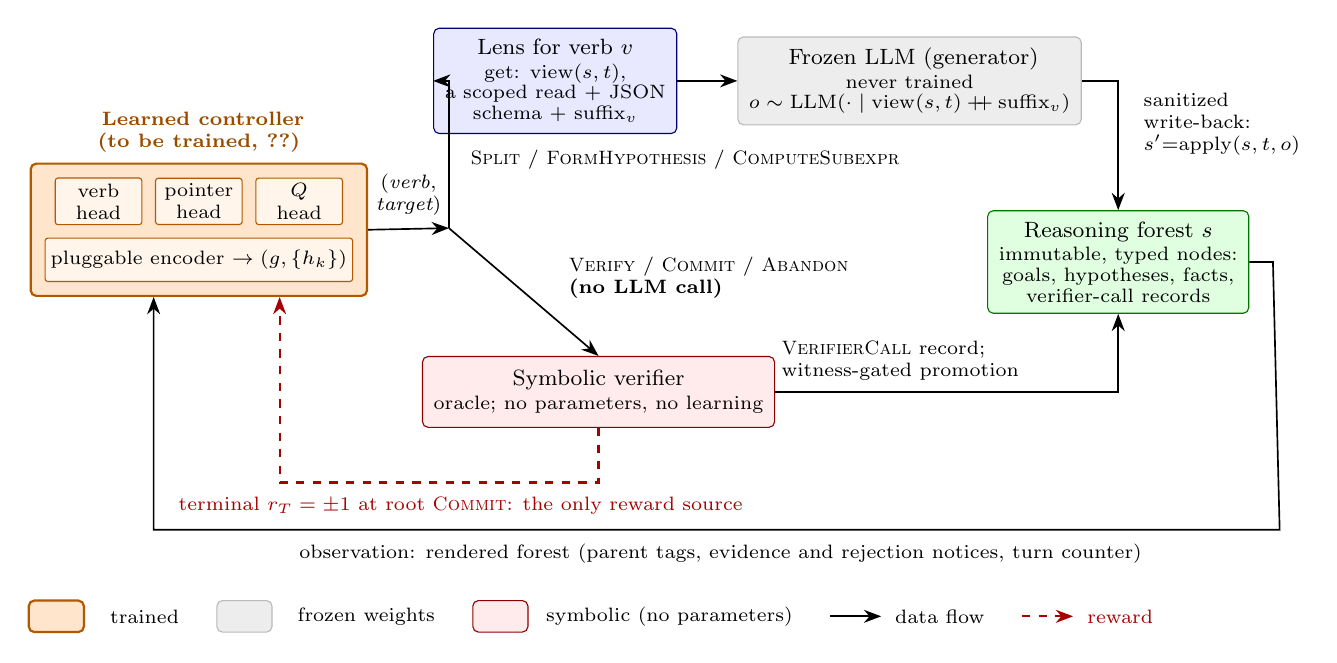
\begin{tikzpicture}[
    font=\footnotesize,
    box/.style={draw, rounded corners=2pt, align=center, inner sep=4pt,
                minimum height=9mm},
    trained/.style={box, fill=orange!20, draw=orange!70!black, thick},
    frozen/.style={box, fill=gray!14, draw=gray!55},
    symbolic/.style={box, fill=red!8, draw=red!55!black},
    state/.style={box, fill=green!12, draw=green!45!black},
    lensbox/.style={box, fill=blue!9, draw=blue!45!black},
    head/.style={draw=orange!70!black, fill=orange!8, rounded corners=1pt,
                 align=center, inner sep=2pt, font=\scriptsize,
                 minimum width=11mm, minimum height=5.5mm},
    lab/.style={font=\scriptsize, align=center},
    arr/.style={-{Stealth[length=2.2mm]}, semithick},
    rew/.style={-{Stealth[length=2.2mm]}, thick, dashed, red!65!black}]

  % ---- learned controller (composite; the only trained component) ----
  \node[head] (verbh) at (0,0.42) {verb\\head};
  \node[head, right=1.6mm of verbh] (ptrh) {pointer\\head};
  \node[head, right=1.6mm of ptrh] (qh) {$Q$\\head};
  \node[head, minimum width=39mm, below=1.6mm of ptrh.south, anchor=north]
    (enc) {pluggable encoder $\to (g, \{h_k\})$};
  \begin{scope}[on background layer]
    \node[trained, fit=(verbh)(ptrh)(qh)(enc), inner sep=5pt,
          label={[font=\scriptsize\bfseries, orange!60!black,
                  align=center]above:{%
            \icontrained\ Learned controller\\
            (to be trained, \cref{sec:training})}}]
      (ctrl) {};
  \end{scope}

  % ---- lens, frozen LLM, forest, verifier ----
  \node[lensbox] (lens) at (5.8,1.95)
    {Lens for verb $v$\\[-1pt]
     \scriptsize get: $\mathrm{view}(s,t)$,\\[-2pt]
     \scriptsize a scoped read $+$ JSON\\[-2pt]
     \scriptsize schema $+$ $\mathrm{suffix}_v$};
  \node[frozen] (llm) at (10.3,1.95)
    {\iconfrozen\ Frozen LLM (generator)\\[-1pt]
     \scriptsize never trained\\[-2pt]
     \scriptsize $o \sim \mathrm{LLM}(\cdot \mid \mathrm{view}(s,t)
       \mathbin{+\!\!+} \mathrm{suffix}_v)$};
  \node[state] (forest) at (12.95,-0.35)
    {Reasoning forest $s$\\[-1pt]
     \scriptsize immutable, typed nodes:\\[-2pt]
     \scriptsize goals, hypotheses, facts,\\[-2pt]
     \scriptsize verifier-call records};
  \node[symbolic] (ver) at (6.35,-2.0)
    {Symbolic verifier\\[-1pt]
     \scriptsize oracle; no parameters, no learning};

  % ---- action fan-out ----
  \coordinate (branch) at (4.45,0.08);
  \draw[arr] (ctrl.east) -- node[lab, above=0.4mm]
    {$(\textit{verb},$\\ $\textit{target})$} (branch);
  \draw[arr] (branch) |- (lens.west);
  \node[lab, anchor=west] at (4.6,0.95)
    {\textsc{Split} / \textsc{FormHypothesis} / \textsc{ComputeSubexpr}};
  \draw[arr] (branch) -- (ver.north);
  \node[lab, anchor=west, align=left] at (5.85,-0.55)
    {\textsc{Verify} / \textsc{Commit} / \textsc{Abandon}\\
     \textbf{(no LLM call)}};

  % ---- generative path ----
  \draw[arr] (lens) -- (llm);
  \draw[arr] (llm.east) -| (forest.north);
  \node[lab, anchor=west, align=left] at (13.15,1.4)
    {sanitized\\ write-back:\\ $s' {=} \mathrm{apply}(s,t,o)$};

  % ---- verifier path into the state ----
  \draw[arr] (ver.east) -| (forest.south);
  \node[lab, anchor=west, align=left] at (8.55,-1.6)
    {\textsc{VerifierCall} record;\\ witness-gated promotion};

  % ---- observation back to the controller (outer loop, bottom) ----
  \draw[arr] (forest.east) -- ++(0.3,0) -- (15.0,-3.75) -- (0.7,-3.75)
    -- (ctrl.south -| 0.7,0);
  \node[lab] at (7.9,-4.05)
    {observation: rendered forest (parent tags, evidence and rejection
     notices, turn counter)};

  % ---- reward (learning signal; the only reward source) ----
  \draw[rew] (ver.south) -- (6.35,-3.15) -- (2.3,-3.15)
    -- (ctrl.south -| 2.3,0);
  \node[lab, red!65!black] at (4.6,-3.45)
    {terminal $r_T = \pm 1$ at root \textsc{Commit}: the only reward source};

  % ---- legend ----
  \begin{scope}[shift={(-0.9,-4.85)}, font=\scriptsize]
    \node[trained, minimum height=4mm, minimum width=7mm, inner sep=1pt,
          anchor=west] (lg1) at (0,0) {};
    \node[right=1mm of lg1, anchor=west] (lg1t) {\icontrained\ trained};
    \node[frozen, minimum height=4mm, minimum width=7mm, inner sep=1pt,
          right=3.5mm of lg1t] (lg2) {};
    \node[right=1mm of lg2, anchor=west] (lg2t)
      {\iconfrozen\ frozen weights};
    \node[symbolic, minimum height=4mm, minimum width=7mm, inner sep=1pt,
          right=3.5mm of lg2t] (lg3) {};
    \node[right=1mm of lg3, anchor=west] (lg3t) {symbolic (no parameters)};
    \draw[arr] ([xshift=3.5mm]lg3t.east) -- ++(0.65,0)
      node[right=0.5mm, anchor=west] (lg4t) {data flow};
    \draw[rew] ([xshift=3.5mm]lg4t.east) -- ++(0.65,0)
      node[right=0.5mm, anchor=west] {reward};
  \end{scope}
\end{tikzpicture}
\caption{One rollout step of the lens-structured context MDP
(\cref{sec:method}). The learned controller (verb head, pointer head, $Q$
head over a pluggable encoder) is the \emph{only} component that is ever
trained; it is untrained at rung 1 and acquires its weights in rungs 2--3 of
\cref{sec:training}. It emits a typed action $a = (\textit{verb},
\textit{target})$. Generative verbs pass through the lens, which renders a
scoped view of the target's neighborhood into the frozen LLM and writes the
sanitized output back into the immutable reasoning forest.
\textsc{Verify}, \textsc{Commit}, and \textsc{Abandon} never call the LLM:
the policy can neither author what is checked nor what it is checked
against. The symbolic verifier is the only reward source (dashed red):
terminal $r_T = \pm 1$ at a root \textsc{Commit}, $0$ at the depth limit
with no root commit, and zero task reward elsewhere (a masked action costs
a constant $-0.01$; \cref{sec:method-reward}). Framing: RL first, MCTS
second; the central object is this agent learning over the induced context
MDP, and MCTS (\cref{fig:training-ladder}) is a strictly additive
accelerator, never the spine.}
\label{fig:architecture}
\end{figure}


\bibliographystyle{plainnat}
\bibliography{references}

\end{document}
